\chapter{Methodology}
\section{SOFTWARE DEVELOPMENT METHODOLOGY}
Agile method \ref{fig:agile_model_for_sdlc} of Software Development uses iterative approach. Agile method cycles among Planning, Designing, Development and Testing stages. These cycle is called sprints. Each sprints are considered as a miniature project on itself. Using this method allows us to update various parts of project at any point of project development.
\begin{figure}[H]
    \centering
    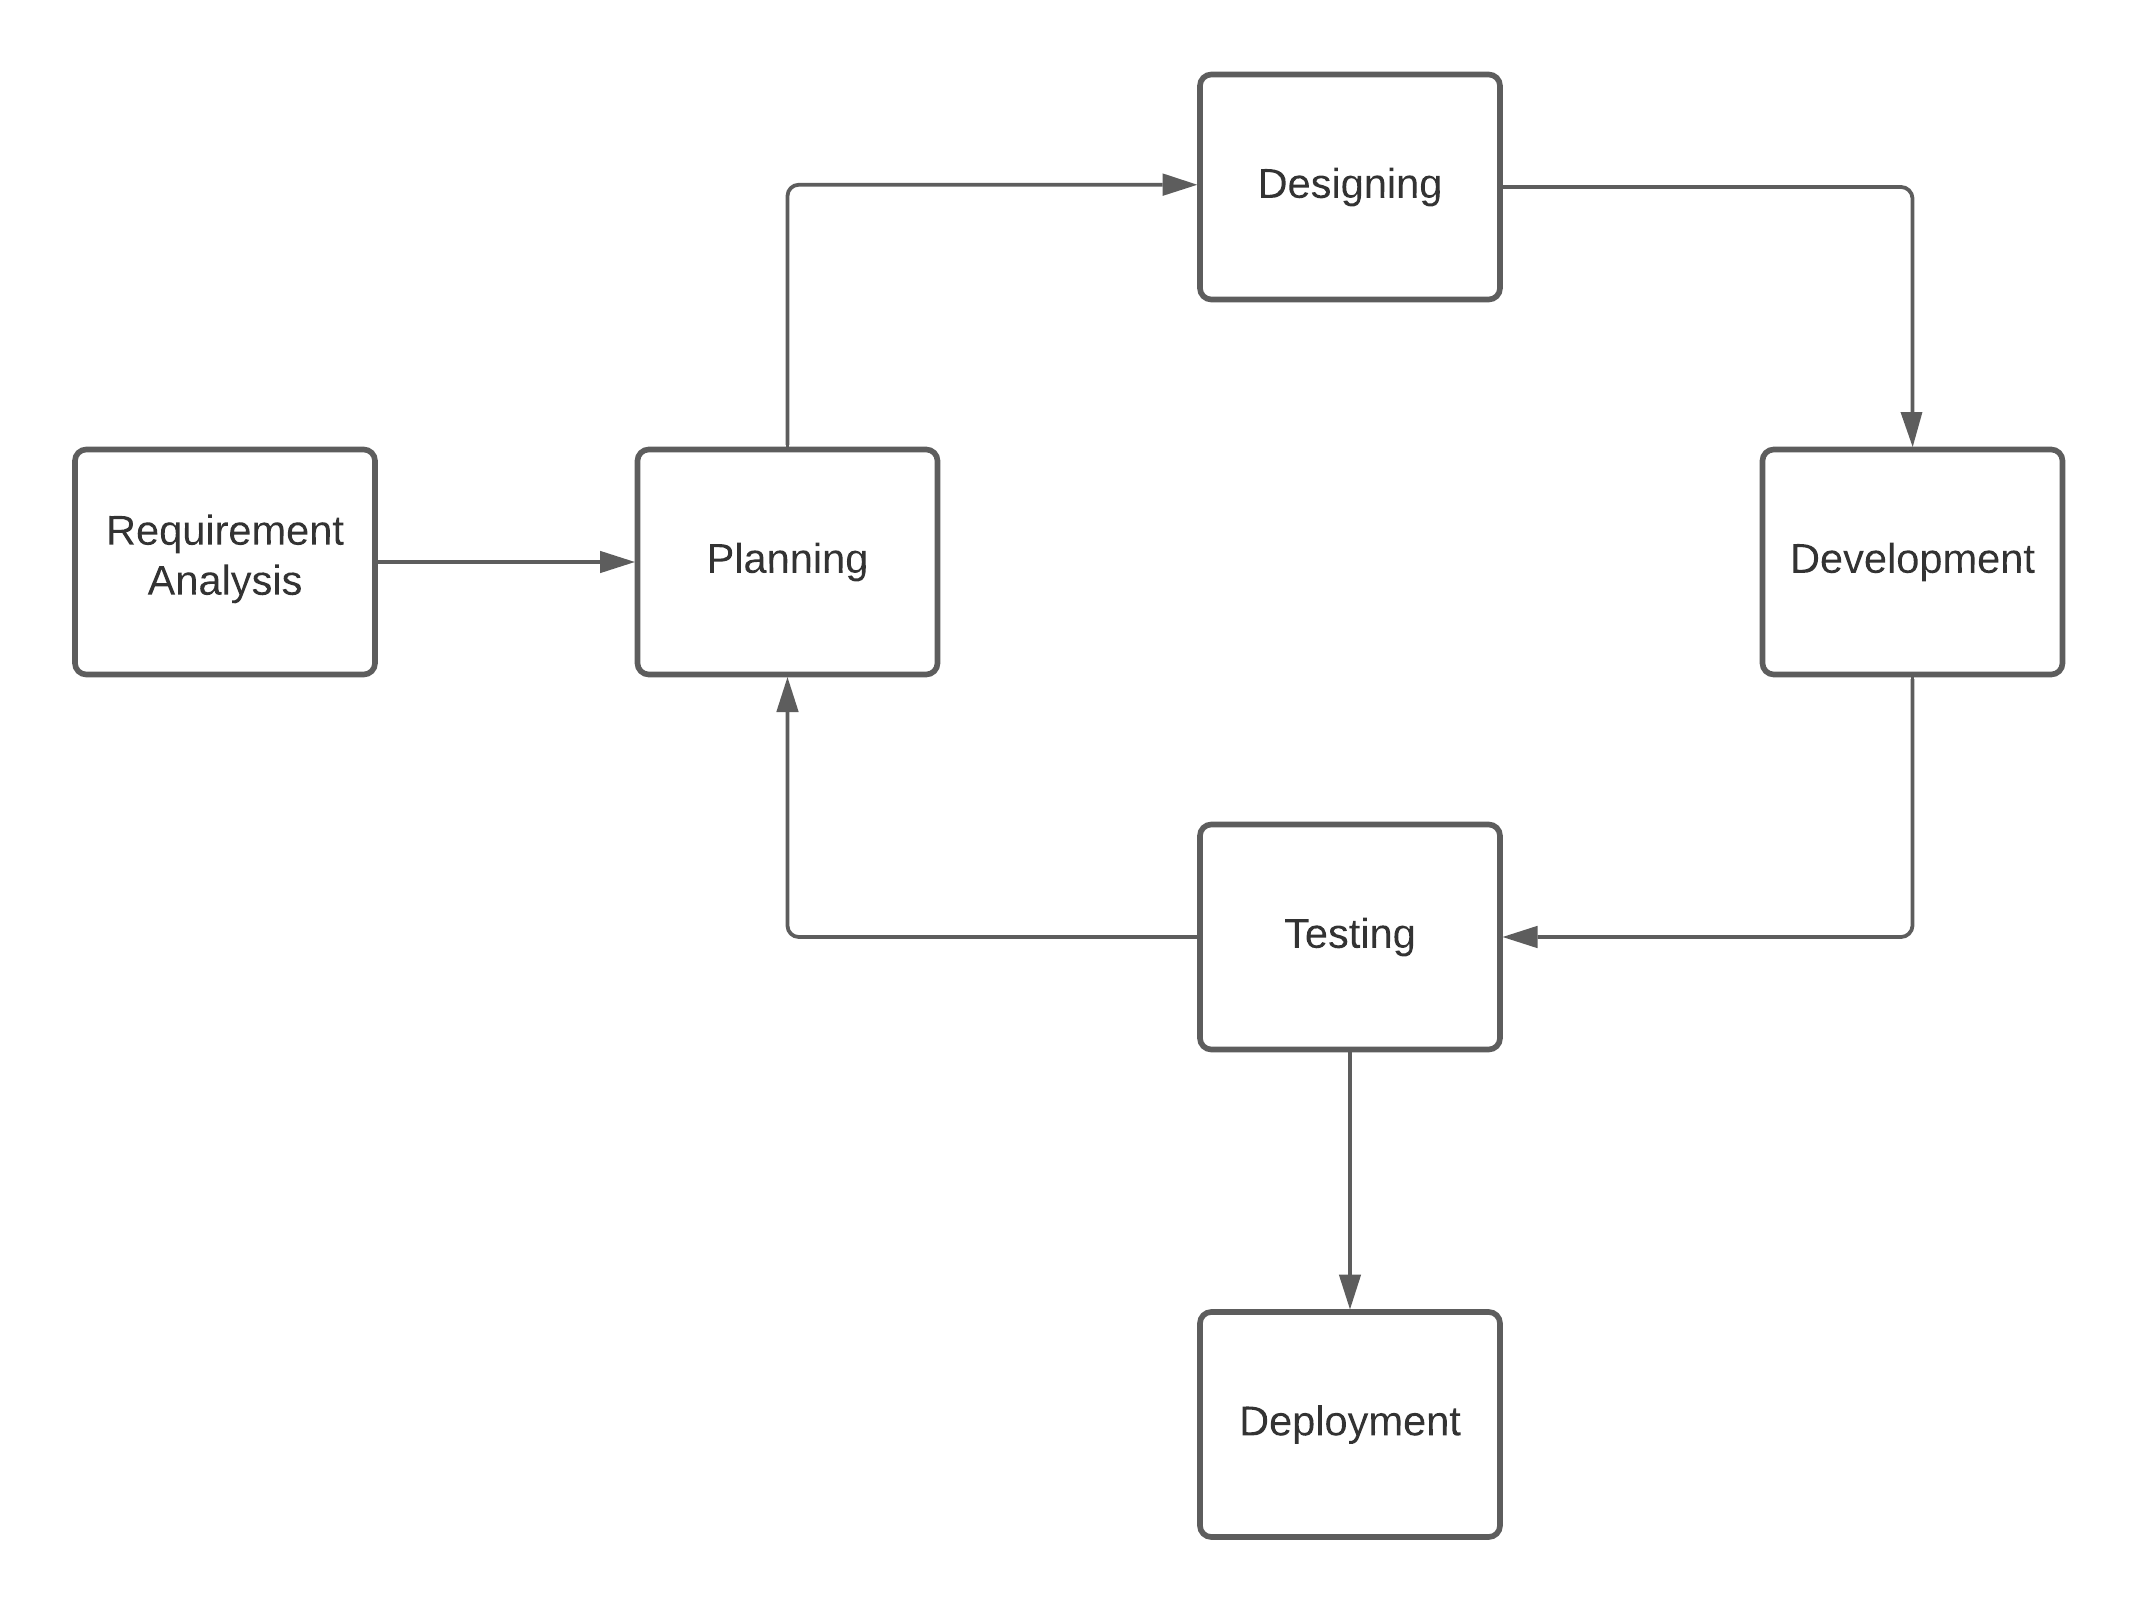
\includegraphics[scale=0.7]{img/AgileMethodology.png}
    \caption{Agile Model For Software Development}
    \label{fig:agile_model_for_sdlc}
\end{figure}
\newpage
\section{Data Collection}
We have collected data from various websites like kaggle.com, github.com and other sources. This data majorly includes Nepali number plate photos and some devanagari
characters in scanned form.

\section{Image Processing}
We process collected data in several sub-processes such as: Colour Space Conversion, Colour Masking, Number-plate Localization, Character Separation, and Character recognition.
\subsection{Number-plate Localization}
In this process we will locate number-pate from the still frame of video-feed and snaps it out for further processing. It snaps rectangular snip of image containing just the number-plate.
\subsection{Colour Space Conversion}
In This process we will convert widely used RGB image format to HSV image format. This allows us to easily recognize colour of the number-plate and hence allows us to classify number-plates into various types such as: Private vehicle, Public Vehicle, Government vehicle, Diplomatic Vehicle, Tourist Vehicle and National Corporation. 
\subsection{Colour Masking}
In this process we will convert snapped image of number-plate in HSV format and recognize general foreground colour by looking at the hue value. By reducing saturation we can easily convert colourful image into monochromatic image. Alongside this depending upon foreground colour we can change hue to get black text on white background.  
\subsection{Character Separation}
Here we will separate different characters onto their own. Thus this black and white single character image can be forwarded for character recognition process.
\subsection{Character recognition}
In this process we will recognize characters separated before one by one to get number-plate data. This process is done using Convoluted Neural Network (CNN) 